\documentclass[12pt,letterpaper]{article}
\usepackage[margin=0.65in,top=0.75in,bottom=0.65in,headheight=15pt,headsep=17pt,footskip=24pt]{geometry}
\usepackage{lmodern}
\pdfmapfile{+lm.map}
\pdfmapfile{+cm.map}
\usepackage{tikz}
\usetikzlibrary{arrows.meta}
\usepackage{fancyhdr}
\renewcommand{\familydefault}{\sfdefault}
\setlength{\parindent}{0pt}
\setlength{\parskip}{7pt}
\pagestyle{fancy}
\fancyhf{}
\renewcommand{\headrulewidth}{0pt}
\renewcommand{\footrulewidth}{0pt}
\fancyhead[L]{\fontsize{11}{13}\selectfont Week 13 / Route packing and bottlenecks / Grades 4--5}
\fancyfoot[L]{\fontsize{9}{11}\selectfont Bellingham Math Circle / Week 13 / F13-45-v2}
\fancyfoot[R]{\fontsize{9}{11}\selectfont\thepage}
\begin{document}
\fontsize{12}{16}\selectfont
A route follows arrows from Start to Finish without visiting a dot twice. Routes may meet at dots, but each arrow can belong to only one route in a collection. Use a different color or line pattern for each route. A marker closes one arrow.
\vspace{0.1in}
\par\textbf{Problem 1:} The thick arrows form reserved routes. No more routes fit beside them. Replace them with a largest collection on each board.

\vspace{0.05in}
\begin{center}
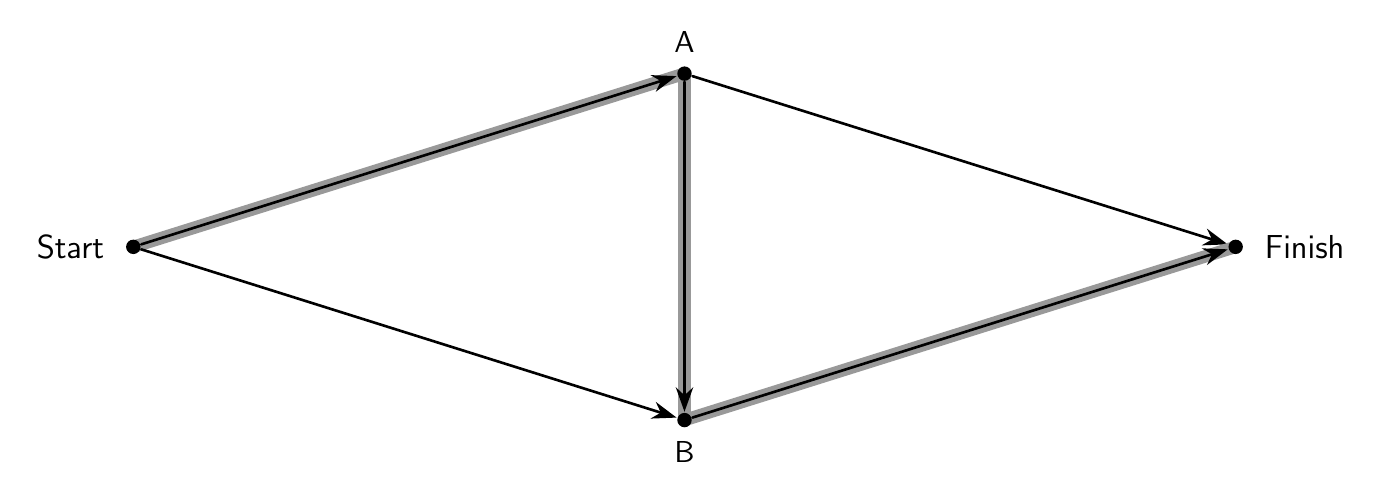
\begin{tikzpicture}[x=1cm,y=1cm,>={Stealth[length=3.1mm,width=2.2mm]},line cap=round,line join=round]
\coordinate (s) at (0,0);
\coordinate (A) at (7,2.2);
\coordinate (B) at (7,-2.2);
\coordinate (t) at (14,0);
\draw[line width=4.5pt,black!40] (s) -- (A);
\draw[->,line width=0.95pt,shorten >=3pt,shorten <=3pt] (s) -- (A);
\draw[->,line width=0.95pt,shorten >=3pt,shorten <=3pt] (s) -- (B);
\draw[line width=4.5pt,black!40] (A) -- (B);
\draw[->,line width=0.95pt,shorten >=3pt,shorten <=3pt] (A) -- (B);
\draw[->,line width=0.95pt,shorten >=3pt,shorten <=3pt] (A) -- (t);
\draw[line width=4.5pt,black!40] (B) -- (t);
\draw[->,line width=0.95pt,shorten >=3pt,shorten <=3pt] (B) -- (t);
\fill (s) circle (2.6pt);
\node[left=7pt,font=\fontsize{12}{14}\selectfont] at (s) {Start};
\fill (A) circle (2.6pt);
\node[above=6pt,fill=white,inner sep=1.4pt,font=\fontsize{11}{12}\selectfont] at (A) {A};
\fill (B) circle (2.6pt);
\node[below=6pt,fill=white,inner sep=1.4pt,font=\fontsize{11}{12}\selectfont] at (B) {B};
\fill (t) circle (2.6pt);
\node[right=7pt,font=\fontsize{12}{14}\selectfont] at (t) {Finish};
\end{tikzpicture}
\end{center}
\vspace{0.32in}
\begin{center}
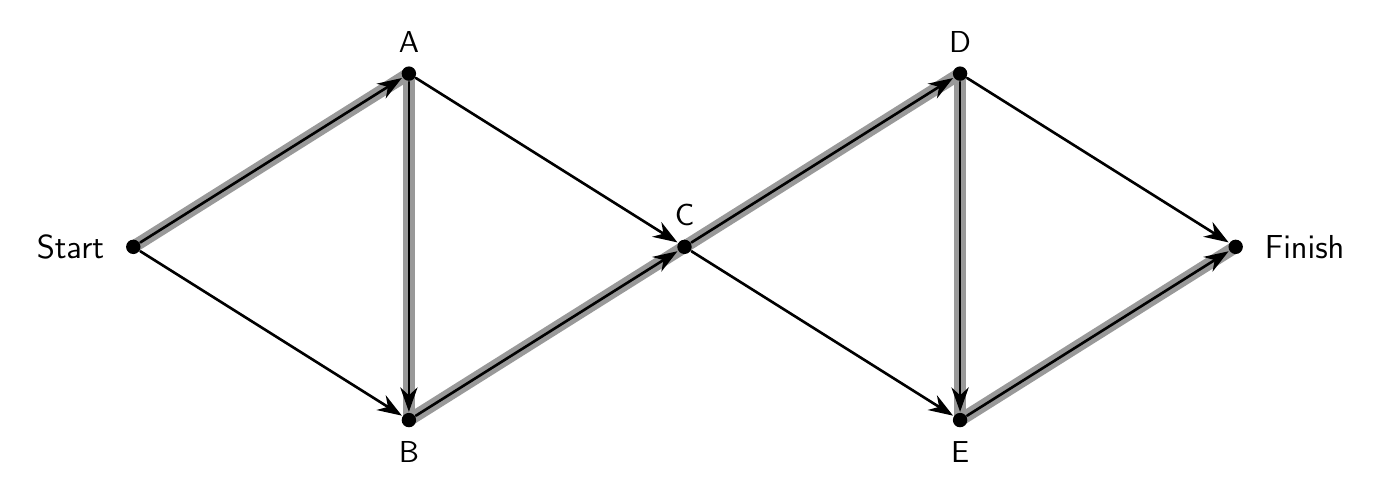
\begin{tikzpicture}[x=1cm,y=1cm,>={Stealth[length=3.1mm,width=2.2mm]},line cap=round,line join=round]
\coordinate (s) at (0,0);
\coordinate (A) at (3.5,2.2);
\coordinate (B) at (3.5,-2.2);
\coordinate (C) at (7,0);
\coordinate (D) at (10.5,2.2);
\coordinate (E) at (10.5,-2.2);
\coordinate (t) at (14,0);
\draw[line width=4.5pt,black!40] (s) -- (A);
\draw[->,line width=0.95pt,shorten >=3pt,shorten <=3pt] (s) -- (A);
\draw[->,line width=0.95pt,shorten >=3pt,shorten <=3pt] (s) -- (B);
\draw[line width=4.5pt,black!40] (A) -- (B);
\draw[->,line width=0.95pt,shorten >=3pt,shorten <=3pt] (A) -- (B);
\draw[->,line width=0.95pt,shorten >=3pt,shorten <=3pt] (A) -- (C);
\draw[line width=4.5pt,black!40] (B) -- (C);
\draw[->,line width=0.95pt,shorten >=3pt,shorten <=3pt] (B) -- (C);
\draw[line width=4.5pt,black!40] (C) -- (D);
\draw[->,line width=0.95pt,shorten >=3pt,shorten <=3pt] (C) -- (D);
\draw[->,line width=0.95pt,shorten >=3pt,shorten <=3pt] (C) -- (E);
\draw[line width=4.5pt,black!40] (D) -- (E);
\draw[->,line width=0.95pt,shorten >=3pt,shorten <=3pt] (D) -- (E);
\draw[->,line width=0.95pt,shorten >=3pt,shorten <=3pt] (D) -- (t);
\draw[line width=4.5pt,black!40] (E) -- (t);
\draw[->,line width=0.95pt,shorten >=3pt,shorten <=3pt] (E) -- (t);
\fill (s) circle (2.6pt);
\node[left=7pt,font=\fontsize{12}{14}\selectfont] at (s) {Start};
\fill (A) circle (2.6pt);
\node[above=6pt,fill=white,inner sep=1.4pt,font=\fontsize{11}{12}\selectfont] at (A) {A};
\fill (B) circle (2.6pt);
\node[below=6pt,fill=white,inner sep=1.4pt,font=\fontsize{11}{12}\selectfont] at (B) {B};
\fill (C) circle (2.6pt);
\node[above=6pt,fill=white,inner sep=1.4pt,font=\fontsize{11}{12}\selectfont] at (C) {C};
\fill (D) circle (2.6pt);
\node[above=6pt,fill=white,inner sep=1.4pt,font=\fontsize{11}{12}\selectfont] at (D) {D};
\fill (E) circle (2.6pt);
\node[below=6pt,fill=white,inner sep=1.4pt,font=\fontsize{11}{12}\selectfont] at (E) {E};
\fill (t) circle (2.6pt);
\node[right=7pt,font=\fontsize{12}{14}\selectfont] at (t) {Finish};
\end{tikzpicture}
\end{center}


\newpage

\vspace{0.05in}
\begin{center}
\begin{tikzpicture}[x=1cm,y=1cm,>={Stealth[length=3.1mm,width=2.2mm]},line cap=round,line join=round]
\coordinate (s) at (0,0);
\coordinate (A) at (7,2.2);
\coordinate (B) at (7,-2.2);
\coordinate (t) at (14,0);
\draw[->,line width=0.95pt,shorten >=3pt,shorten <=3pt] (s) -- (A);
\draw[->,line width=0.95pt,shorten >=3pt,shorten <=3pt] (s) -- (B);
\draw[->,line width=0.95pt,shorten >=3pt,shorten <=3pt] (A) -- (B);
\draw[->,line width=0.95pt,shorten >=3pt,shorten <=3pt] (A) -- (t);
\draw[->,line width=0.95pt,shorten >=3pt,shorten <=3pt] (B) -- (t);
\fill (s) circle (2.6pt);
\node[left=7pt,font=\fontsize{12}{14}\selectfont] at (s) {Start};
\fill (A) circle (2.6pt);
\node[above=6pt,fill=white,inner sep=1.4pt,font=\fontsize{11}{12}\selectfont] at (A) {A};
\fill (B) circle (2.6pt);
\node[below=6pt,fill=white,inner sep=1.4pt,font=\fontsize{11}{12}\selectfont] at (B) {B};
\fill (t) circle (2.6pt);
\node[right=7pt,font=\fontsize{12}{14}\selectfont] at (t) {Finish};
\end{tikzpicture}
\end{center}
\vspace{0.32in}
\begin{center}
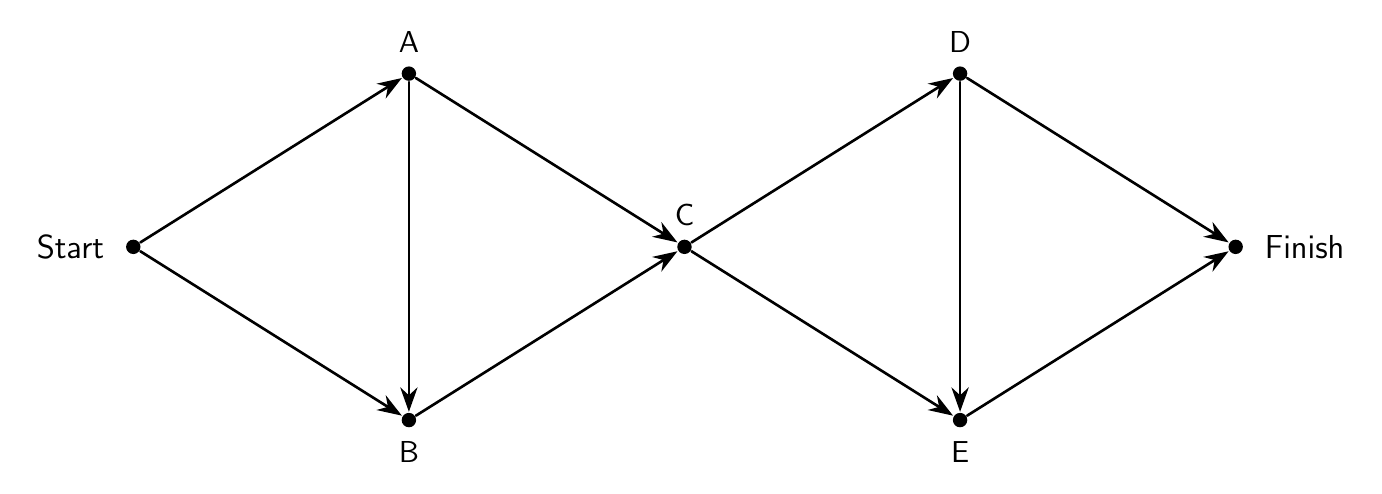
\begin{tikzpicture}[x=1cm,y=1cm,>={Stealth[length=3.1mm,width=2.2mm]},line cap=round,line join=round]
\coordinate (s) at (0,0);
\coordinate (A) at (3.5,2.2);
\coordinate (B) at (3.5,-2.2);
\coordinate (C) at (7,0);
\coordinate (D) at (10.5,2.2);
\coordinate (E) at (10.5,-2.2);
\coordinate (t) at (14,0);
\draw[->,line width=0.95pt,shorten >=3pt,shorten <=3pt] (s) -- (A);
\draw[->,line width=0.95pt,shorten >=3pt,shorten <=3pt] (s) -- (B);
\draw[->,line width=0.95pt,shorten >=3pt,shorten <=3pt] (A) -- (B);
\draw[->,line width=0.95pt,shorten >=3pt,shorten <=3pt] (A) -- (C);
\draw[->,line width=0.95pt,shorten >=3pt,shorten <=3pt] (B) -- (C);
\draw[->,line width=0.95pt,shorten >=3pt,shorten <=3pt] (C) -- (D);
\draw[->,line width=0.95pt,shorten >=3pt,shorten <=3pt] (C) -- (E);
\draw[->,line width=0.95pt,shorten >=3pt,shorten <=3pt] (D) -- (E);
\draw[->,line width=0.95pt,shorten >=3pt,shorten <=3pt] (D) -- (t);
\draw[->,line width=0.95pt,shorten >=3pt,shorten <=3pt] (E) -- (t);
\fill (s) circle (2.6pt);
\node[left=7pt,font=\fontsize{12}{14}\selectfont] at (s) {Start};
\fill (A) circle (2.6pt);
\node[above=6pt,fill=white,inner sep=1.4pt,font=\fontsize{11}{12}\selectfont] at (A) {A};
\fill (B) circle (2.6pt);
\node[below=6pt,fill=white,inner sep=1.4pt,font=\fontsize{11}{12}\selectfont] at (B) {B};
\fill (C) circle (2.6pt);
\node[above=6pt,fill=white,inner sep=1.4pt,font=\fontsize{11}{12}\selectfont] at (C) {C};
\fill (D) circle (2.6pt);
\node[above=6pt,fill=white,inner sep=1.4pt,font=\fontsize{11}{12}\selectfont] at (D) {D};
\fill (E) circle (2.6pt);
\node[below=6pt,fill=white,inner sep=1.4pt,font=\fontsize{11}{12}\selectfont] at (E) {E};
\fill (t) circle (2.6pt);
\node[right=7pt,font=\fontsize{12}{14}\selectfont] at (t) {Finish};
\end{tikzpicture}
\end{center}


\newpage
\par\textbf{Problem 2:} Find a largest route collection and a smallest set of closing arrows. Explain why your closing arrows stop every route and why the two answers show that your collection is largest.

\vspace{0.26in}
\begin{center}
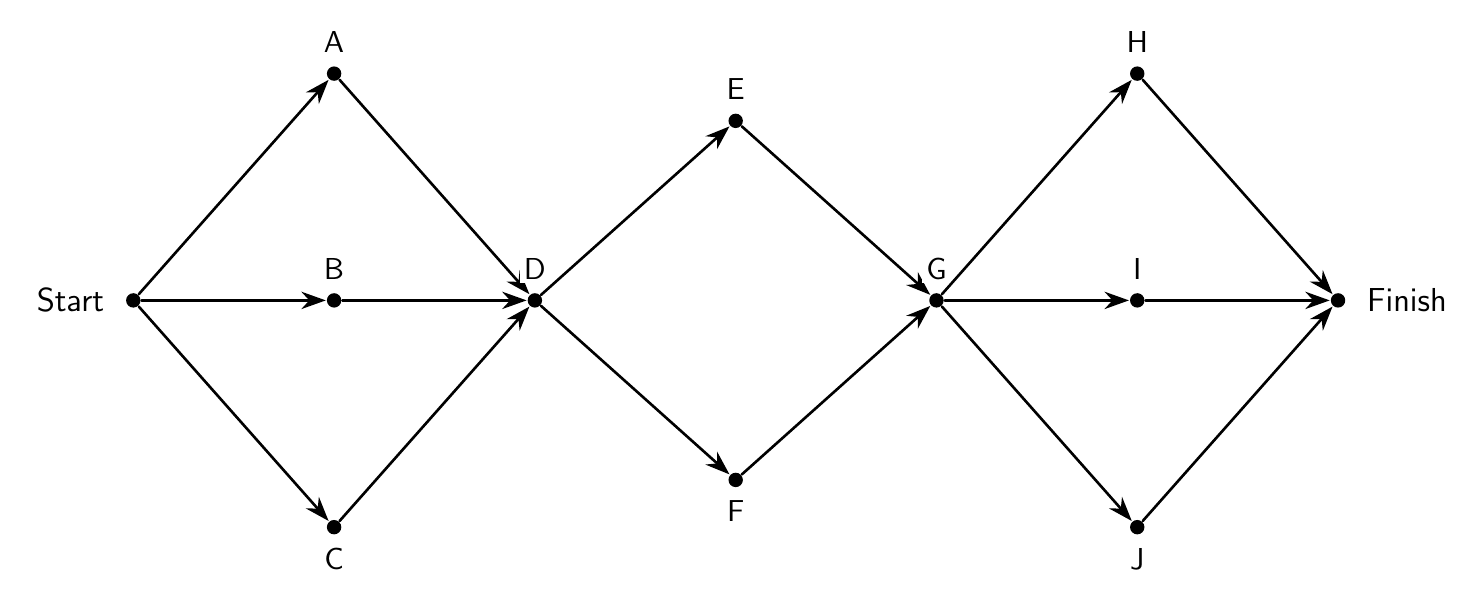
\begin{tikzpicture}[x=1.02cm,y=1.2cm,>={Stealth[length=3.1mm,width=2.2mm]},line cap=round,line join=round]
\coordinate (s) at (0,0);
\coordinate (A) at (2.5,2.4);
\coordinate (B) at (2.5,0);
\coordinate (C) at (2.5,-2.4);
\coordinate (D) at (5,0);
\coordinate (E) at (7.5,1.9);
\coordinate (F) at (7.5,-1.9);
\coordinate (G) at (10,0);
\coordinate (H) at (12.5,2.4);
\coordinate (I) at (12.5,0);
\coordinate (J) at (12.5,-2.4);
\coordinate (t) at (15,0);
\draw[->,line width=0.95pt,shorten >=3pt,shorten <=3pt] (s) -- (A);
\draw[->,line width=0.95pt,shorten >=3pt,shorten <=3pt] (s) -- (B);
\draw[->,line width=0.95pt,shorten >=3pt,shorten <=3pt] (s) -- (C);
\draw[->,line width=0.95pt,shorten >=3pt,shorten <=3pt] (A) -- (D);
\draw[->,line width=0.95pt,shorten >=3pt,shorten <=3pt] (B) -- (D);
\draw[->,line width=0.95pt,shorten >=3pt,shorten <=3pt] (C) -- (D);
\draw[->,line width=0.95pt,shorten >=3pt,shorten <=3pt] (D) -- (E);
\draw[->,line width=0.95pt,shorten >=3pt,shorten <=3pt] (D) -- (F);
\draw[->,line width=0.95pt,shorten >=3pt,shorten <=3pt] (E) -- (G);
\draw[->,line width=0.95pt,shorten >=3pt,shorten <=3pt] (F) -- (G);
\draw[->,line width=0.95pt,shorten >=3pt,shorten <=3pt] (G) -- (H);
\draw[->,line width=0.95pt,shorten >=3pt,shorten <=3pt] (G) -- (I);
\draw[->,line width=0.95pt,shorten >=3pt,shorten <=3pt] (G) -- (J);
\draw[->,line width=0.95pt,shorten >=3pt,shorten <=3pt] (H) -- (t);
\draw[->,line width=0.95pt,shorten >=3pt,shorten <=3pt] (I) -- (t);
\draw[->,line width=0.95pt,shorten >=3pt,shorten <=3pt] (J) -- (t);
\fill (s) circle (2.6pt);
\node[left=7pt,font=\fontsize{12}{14}\selectfont] at (s) {Start};
\fill (A) circle (2.6pt);
\node[above=6pt,fill=white,inner sep=1.4pt,font=\fontsize{11}{12}\selectfont] at (A) {A};
\fill (B) circle (2.6pt);
\node[above=6pt,fill=white,inner sep=1.4pt,font=\fontsize{11}{12}\selectfont] at (B) {B};
\fill (C) circle (2.6pt);
\node[below=6pt,fill=white,inner sep=1.4pt,font=\fontsize{11}{12}\selectfont] at (C) {C};
\fill (D) circle (2.6pt);
\node[above=6pt,fill=white,inner sep=1.4pt,font=\fontsize{11}{12}\selectfont] at (D) {D};
\fill (E) circle (2.6pt);
\node[above=6pt,fill=white,inner sep=1.4pt,font=\fontsize{11}{12}\selectfont] at (E) {E};
\fill (F) circle (2.6pt);
\node[below=6pt,fill=white,inner sep=1.4pt,font=\fontsize{11}{12}\selectfont] at (F) {F};
\fill (G) circle (2.6pt);
\node[above=6pt,fill=white,inner sep=1.4pt,font=\fontsize{11}{12}\selectfont] at (G) {G};
\fill (H) circle (2.6pt);
\node[above=6pt,fill=white,inner sep=1.4pt,font=\fontsize{11}{12}\selectfont] at (H) {H};
\fill (I) circle (2.6pt);
\node[above=6pt,fill=white,inner sep=1.4pt,font=\fontsize{11}{12}\selectfont] at (I) {I};
\fill (J) circle (2.6pt);
\node[below=6pt,fill=white,inner sep=1.4pt,font=\fontsize{11}{12}\selectfont] at (J) {J};
\fill (t) circle (2.6pt);
\node[right=7pt,font=\fontsize{12}{14}\selectfont] at (t) {Finish};
\end{tikzpicture}
\end{center}


\newpage
\par\textbf{Problem 3:} Split the dots into two sides, with Start on one side and Finish on the other. The arrows pointing from the Start side to the Finish side are called the cut arrows. Find two different splits with exactly two cut arrows and at least one arrow pointing back into the Start side. Explain why closing the cut arrows stops all travel.

\vspace{0.26in}
\begin{center}
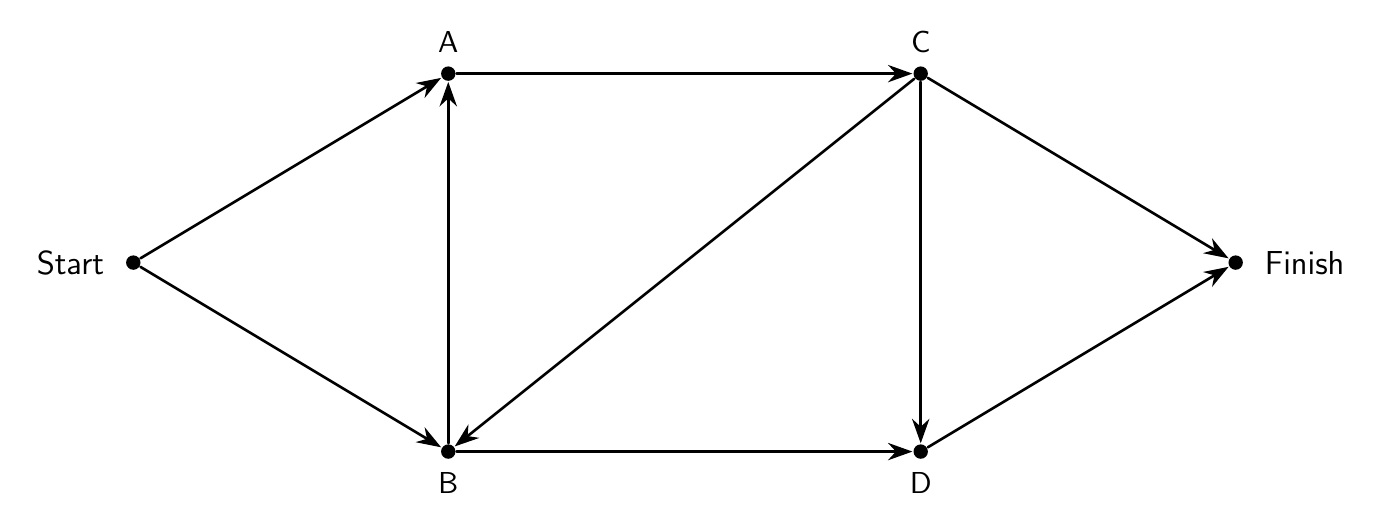
\begin{tikzpicture}[x=1cm,y=1cm,>={Stealth[length=3.1mm,width=2.2mm]},line cap=round,line join=round]
\coordinate (s) at (0,0);
\coordinate (A) at (4,2.4);
\coordinate (B) at (4,-2.4);
\coordinate (C) at (10,2.4);
\coordinate (D) at (10,-2.4);
\coordinate (t) at (14,0);
\draw[->,line width=0.95pt,shorten >=3pt,shorten <=3pt] (s) -- (A);
\draw[->,line width=0.95pt,shorten >=3pt,shorten <=3pt] (s) -- (B);
\draw[->,line width=0.95pt,shorten >=3pt,shorten <=3pt] (A) -- (C);
\draw[->,line width=0.95pt,shorten >=3pt,shorten <=3pt] (B) -- (D);
\draw[->,line width=0.95pt,shorten >=3pt,shorten <=3pt] (C) -- (t);
\draw[->,line width=0.95pt,shorten >=3pt,shorten <=3pt] (D) -- (t);
\draw[->,line width=0.95pt,shorten >=3pt,shorten <=3pt] (B) -- (A);
\draw[->,line width=0.95pt,shorten >=3pt,shorten <=3pt] (C) -- (D);
\draw[->,line width=0.95pt,shorten >=3pt,shorten <=3pt] (C) -- (B);
\fill (s) circle (2.6pt);
\node[left=7pt,font=\fontsize{12}{14}\selectfont] at (s) {Start};
\fill (A) circle (2.6pt);
\node[above=6pt,fill=white,inner sep=1.4pt,font=\fontsize{11}{12}\selectfont] at (A) {A};
\fill (B) circle (2.6pt);
\node[below=6pt,fill=white,inner sep=1.4pt,font=\fontsize{11}{12}\selectfont] at (B) {B};
\fill (C) circle (2.6pt);
\node[above=6pt,fill=white,inner sep=1.4pt,font=\fontsize{11}{12}\selectfont] at (C) {C};
\fill (D) circle (2.6pt);
\node[below=6pt,fill=white,inner sep=1.4pt,font=\fontsize{11}{12}\selectfont] at (D) {D};
\fill (t) circle (2.6pt);
\node[right=7pt,font=\fontsize{12}{14}\selectfont] at (t) {Finish};
\end{tikzpicture}
\end{center}
\vspace{0.32in}
\begin{center}
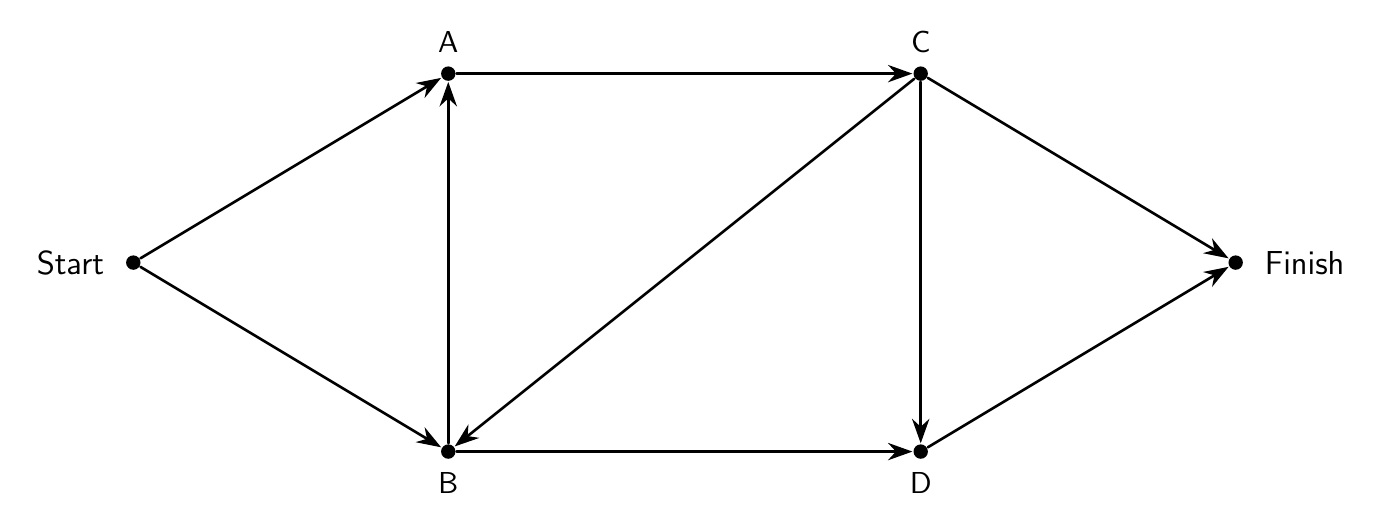
\begin{tikzpicture}[x=1cm,y=1cm,>={Stealth[length=3.1mm,width=2.2mm]},line cap=round,line join=round]
\coordinate (s) at (0,0);
\coordinate (A) at (4,2.4);
\coordinate (B) at (4,-2.4);
\coordinate (C) at (10,2.4);
\coordinate (D) at (10,-2.4);
\coordinate (t) at (14,0);
\draw[->,line width=0.95pt,shorten >=3pt,shorten <=3pt] (s) -- (A);
\draw[->,line width=0.95pt,shorten >=3pt,shorten <=3pt] (s) -- (B);
\draw[->,line width=0.95pt,shorten >=3pt,shorten <=3pt] (A) -- (C);
\draw[->,line width=0.95pt,shorten >=3pt,shorten <=3pt] (B) -- (D);
\draw[->,line width=0.95pt,shorten >=3pt,shorten <=3pt] (C) -- (t);
\draw[->,line width=0.95pt,shorten >=3pt,shorten <=3pt] (D) -- (t);
\draw[->,line width=0.95pt,shorten >=3pt,shorten <=3pt] (B) -- (A);
\draw[->,line width=0.95pt,shorten >=3pt,shorten <=3pt] (C) -- (D);
\draw[->,line width=0.95pt,shorten >=3pt,shorten <=3pt] (C) -- (B);
\fill (s) circle (2.6pt);
\node[left=7pt,font=\fontsize{12}{14}\selectfont] at (s) {Start};
\fill (A) circle (2.6pt);
\node[above=6pt,fill=white,inner sep=1.4pt,font=\fontsize{11}{12}\selectfont] at (A) {A};
\fill (B) circle (2.6pt);
\node[below=6pt,fill=white,inner sep=1.4pt,font=\fontsize{11}{12}\selectfont] at (B) {B};
\fill (C) circle (2.6pt);
\node[above=6pt,fill=white,inner sep=1.4pt,font=\fontsize{11}{12}\selectfont] at (C) {C};
\fill (D) circle (2.6pt);
\node[below=6pt,fill=white,inner sep=1.4pt,font=\fontsize{11}{12}\selectfont] at (D) {D};
\fill (t) circle (2.6pt);
\node[right=7pt,font=\fontsize{12}{14}\selectfont] at (t) {Finish};
\end{tikzpicture}
\end{center}


\newpage
\par\textbf{Problem 4:} Find a smallest set of closing arrows and a route that uses two of those arrows. Can that route belong to a largest collection on this board? Explain.

\vspace{0.26in}
\begin{center}
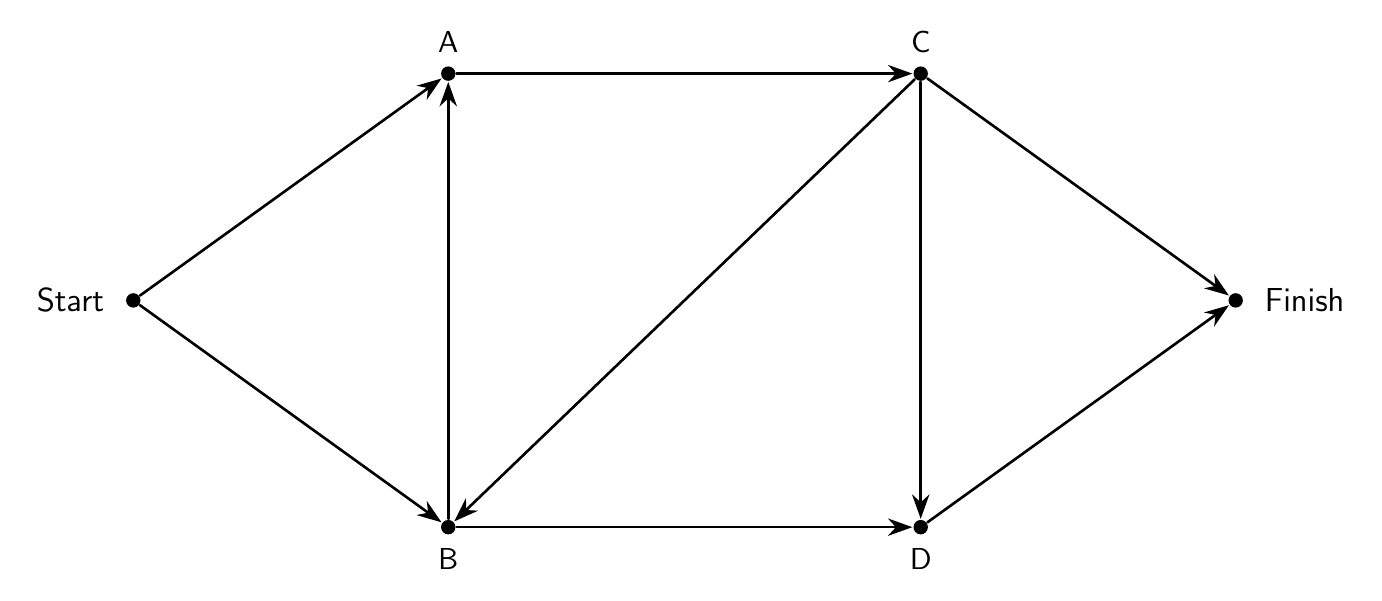
\begin{tikzpicture}[x=1cm,y=1.2cm,>={Stealth[length=3.1mm,width=2.2mm]},line cap=round,line join=round]
\coordinate (s) at (0,0);
\coordinate (A) at (4,2.4);
\coordinate (B) at (4,-2.4);
\coordinate (C) at (10,2.4);
\coordinate (D) at (10,-2.4);
\coordinate (t) at (14,0);
\draw[->,line width=0.95pt,shorten >=3pt,shorten <=3pt] (s) -- (A);
\draw[->,line width=0.95pt,shorten >=3pt,shorten <=3pt] (s) -- (B);
\draw[->,line width=0.95pt,shorten >=3pt,shorten <=3pt] (A) -- (C);
\draw[->,line width=0.95pt,shorten >=3pt,shorten <=3pt] (B) -- (D);
\draw[->,line width=0.95pt,shorten >=3pt,shorten <=3pt] (C) -- (t);
\draw[->,line width=0.95pt,shorten >=3pt,shorten <=3pt] (D) -- (t);
\draw[->,line width=0.95pt,shorten >=3pt,shorten <=3pt] (B) -- (A);
\draw[->,line width=0.95pt,shorten >=3pt,shorten <=3pt] (C) -- (D);
\draw[->,line width=0.95pt,shorten >=3pt,shorten <=3pt] (C) -- (B);
\fill (s) circle (2.6pt);
\node[left=7pt,font=\fontsize{12}{14}\selectfont] at (s) {Start};
\fill (A) circle (2.6pt);
\node[above=6pt,fill=white,inner sep=1.4pt,font=\fontsize{11}{12}\selectfont] at (A) {A};
\fill (B) circle (2.6pt);
\node[below=6pt,fill=white,inner sep=1.4pt,font=\fontsize{11}{12}\selectfont] at (B) {B};
\fill (C) circle (2.6pt);
\node[above=6pt,fill=white,inner sep=1.4pt,font=\fontsize{11}{12}\selectfont] at (C) {C};
\fill (D) circle (2.6pt);
\node[below=6pt,fill=white,inner sep=1.4pt,font=\fontsize{11}{12}\selectfont] at (D) {D};
\fill (t) circle (2.6pt);
\node[right=7pt,font=\fontsize{12}{14}\selectfont] at (t) {Finish};
\end{tikzpicture}
\end{center}


\newpage
A change-walk follows an unused arrow forward or a reserved arrow backward. A forward step reserves its arrow; a backward step cancels its reservation. A change-walk visits each dot at most once. Final routes follow the printed arrows.
\vspace{0.1in}
\begin{center}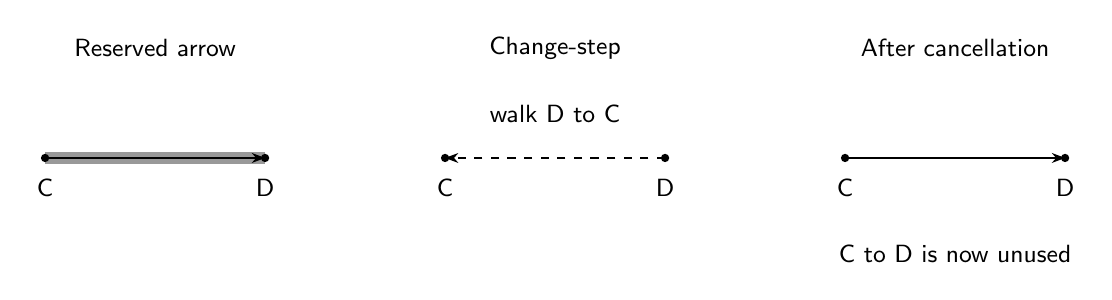
\begin{tikzpicture}[x=1in,y=1in,>=Stealth]
\node[font=\small] at (.7,.55) {Reserved arrow};
\node[font=\small] at (2.7,.55) {Change-step};
\node[font=\small] at (4.7,.55) {After cancellation};
\draw[black!40,line width=4pt] (.15,0)--(1.25,0);
\draw[->] (.15,0)--(1.25,0);
\draw[->,dashed] (3.25,0)--(2.15,0);
\draw[->] (4.15,0)--(5.25,0);
\foreach \x/\t in {.15/C,1.25/D,2.15/C,3.25/D,4.15/C,5.25/D}{\fill (\x,0) circle(1.5pt);\node[below=4pt,font=\small] at (\x,0){\t};}
\node[font=\small] at (2.7,.22) {walk D to C};
\node[font=\small] at (4.7,-.48) {C to D is now unused};
\end{tikzpicture}\end{center}
\par\textbf{Problem 5:} Find a change-walk from Start to Finish that increases the number of routes by one. Draw the resulting route collection.

\vspace{0.02in}
\begin{center}
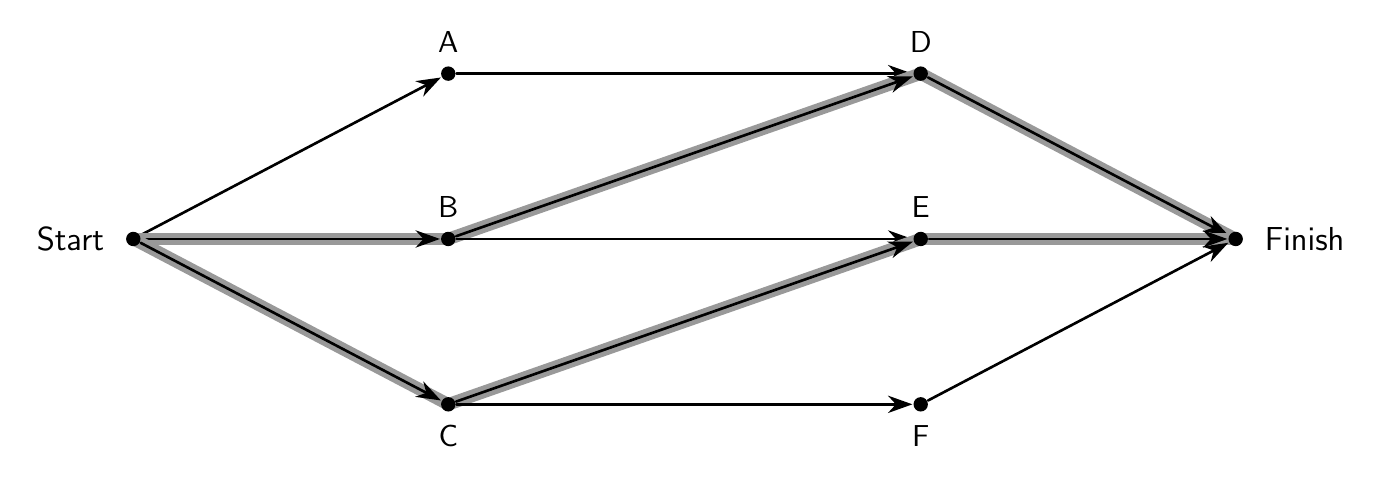
\begin{tikzpicture}[x=1cm,y=0.84cm,>={Stealth[length=3.1mm,width=2.2mm]},line cap=round,line join=round]
\coordinate (s) at (0,0);
\coordinate (A) at (4,2.5);
\coordinate (B) at (4,0);
\coordinate (C) at (4,-2.5);
\coordinate (D) at (10,2.5);
\coordinate (E) at (10,0);
\coordinate (F) at (10,-2.5);
\coordinate (t) at (14,0);
\draw[->,line width=0.95pt,shorten >=3pt,shorten <=3pt] (s) -- (A);
\draw[line width=4.5pt,black!40] (s) -- (B);
\draw[->,line width=0.95pt,shorten >=3pt,shorten <=3pt] (s) -- (B);
\draw[line width=4.5pt,black!40] (s) -- (C);
\draw[->,line width=0.95pt,shorten >=3pt,shorten <=3pt] (s) -- (C);
\draw[->,line width=0.95pt,shorten >=3pt,shorten <=3pt] (A) -- (D);
\draw[line width=4.5pt,black!40] (B) -- (D);
\draw[->,line width=0.95pt,shorten >=3pt,shorten <=3pt] (B) -- (D);
\draw[->,line width=0.95pt,shorten >=3pt,shorten <=3pt] (B) -- (E);
\draw[line width=4.5pt,black!40] (C) -- (E);
\draw[->,line width=0.95pt,shorten >=3pt,shorten <=3pt] (C) -- (E);
\draw[->,line width=0.95pt,shorten >=3pt,shorten <=3pt] (C) -- (F);
\draw[line width=4.5pt,black!40] (D) -- (t);
\draw[->,line width=0.95pt,shorten >=3pt,shorten <=3pt] (D) -- (t);
\draw[line width=4.5pt,black!40] (E) -- (t);
\draw[->,line width=0.95pt,shorten >=3pt,shorten <=3pt] (E) -- (t);
\draw[->,line width=0.95pt,shorten >=3pt,shorten <=3pt] (F) -- (t);
\fill (s) circle (2.6pt);
\node[left=7pt,font=\fontsize{12}{14}\selectfont] at (s) {Start};
\fill (A) circle (2.6pt);
\node[above=6pt,fill=white,inner sep=1.4pt,font=\fontsize{11}{12}\selectfont] at (A) {A};
\fill (B) circle (2.6pt);
\node[above=6pt,fill=white,inner sep=1.4pt,font=\fontsize{11}{12}\selectfont] at (B) {B};
\fill (C) circle (2.6pt);
\node[below=6pt,fill=white,inner sep=1.4pt,font=\fontsize{11}{12}\selectfont] at (C) {C};
\fill (D) circle (2.6pt);
\node[above=6pt,fill=white,inner sep=1.4pt,font=\fontsize{11}{12}\selectfont] at (D) {D};
\fill (E) circle (2.6pt);
\node[above=6pt,fill=white,inner sep=1.4pt,font=\fontsize{11}{12}\selectfont] at (E) {E};
\fill (F) circle (2.6pt);
\node[below=6pt,fill=white,inner sep=1.4pt,font=\fontsize{11}{12}\selectfont] at (F) {F};
\fill (t) circle (2.6pt);
\node[right=7pt,font=\fontsize{12}{14}\selectfont] at (t) {Finish};
\end{tikzpicture}
\end{center}
\vspace{0.32in}
\begin{center}
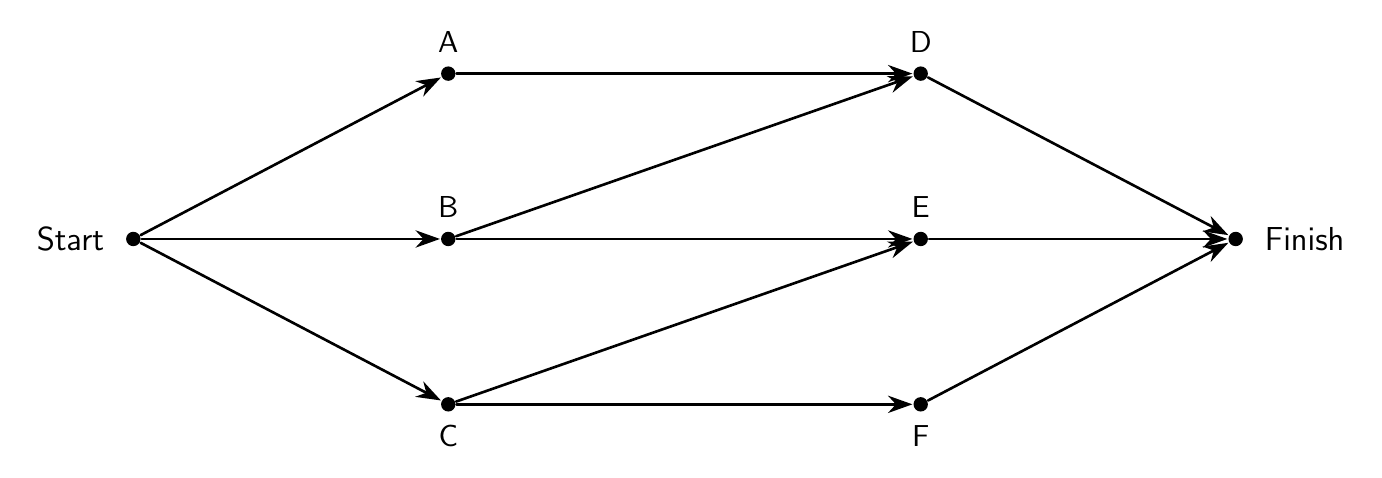
\begin{tikzpicture}[x=1cm,y=0.84cm,>={Stealth[length=3.1mm,width=2.2mm]},line cap=round,line join=round]
\coordinate (s) at (0,0);
\coordinate (A) at (4,2.5);
\coordinate (B) at (4,0);
\coordinate (C) at (4,-2.5);
\coordinate (D) at (10,2.5);
\coordinate (E) at (10,0);
\coordinate (F) at (10,-2.5);
\coordinate (t) at (14,0);
\draw[->,line width=0.95pt,shorten >=3pt,shorten <=3pt] (s) -- (A);
\draw[->,line width=0.95pt,shorten >=3pt,shorten <=3pt] (s) -- (B);
\draw[->,line width=0.95pt,shorten >=3pt,shorten <=3pt] (s) -- (C);
\draw[->,line width=0.95pt,shorten >=3pt,shorten <=3pt] (A) -- (D);
\draw[->,line width=0.95pt,shorten >=3pt,shorten <=3pt] (B) -- (D);
\draw[->,line width=0.95pt,shorten >=3pt,shorten <=3pt] (B) -- (E);
\draw[->,line width=0.95pt,shorten >=3pt,shorten <=3pt] (C) -- (E);
\draw[->,line width=0.95pt,shorten >=3pt,shorten <=3pt] (C) -- (F);
\draw[->,line width=0.95pt,shorten >=3pt,shorten <=3pt] (D) -- (t);
\draw[->,line width=0.95pt,shorten >=3pt,shorten <=3pt] (E) -- (t);
\draw[->,line width=0.95pt,shorten >=3pt,shorten <=3pt] (F) -- (t);
\fill (s) circle (2.6pt);
\node[left=7pt,font=\fontsize{12}{14}\selectfont] at (s) {Start};
\fill (A) circle (2.6pt);
\node[above=6pt,fill=white,inner sep=1.4pt,font=\fontsize{11}{12}\selectfont] at (A) {A};
\fill (B) circle (2.6pt);
\node[above=6pt,fill=white,inner sep=1.4pt,font=\fontsize{11}{12}\selectfont] at (B) {B};
\fill (C) circle (2.6pt);
\node[below=6pt,fill=white,inner sep=1.4pt,font=\fontsize{11}{12}\selectfont] at (C) {C};
\fill (D) circle (2.6pt);
\node[above=6pt,fill=white,inner sep=1.4pt,font=\fontsize{11}{12}\selectfont] at (D) {D};
\fill (E) circle (2.6pt);
\node[above=6pt,fill=white,inner sep=1.4pt,font=\fontsize{11}{12}\selectfont] at (E) {E};
\fill (F) circle (2.6pt);
\node[below=6pt,fill=white,inner sep=1.4pt,font=\fontsize{11}{12}\selectfont] at (F) {F};
\fill (t) circle (2.6pt);
\node[right=7pt,font=\fontsize{12}{14}\selectfont] at (t) {Finish};
\end{tikzpicture}
\end{center}


\newpage
\par\textbf{Problem 6:} The thick arrows form two reserved routes. Find every dot you can reach from Start by change-walk steps. Find a smallest set of closing arrows, and explain why it matches the route collection.

\vspace{0.26in}
\begin{center}
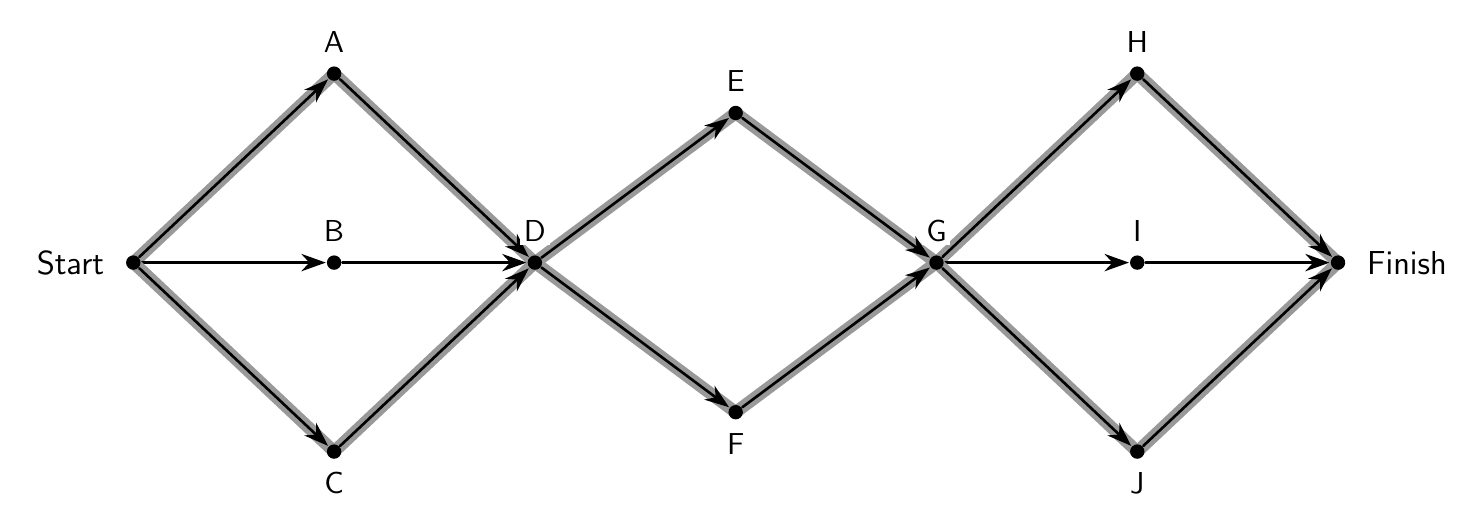
\begin{tikzpicture}[x=1.02cm,y=1cm,>={Stealth[length=3.1mm,width=2.2mm]},line cap=round,line join=round]
\coordinate (s) at (0,0);
\coordinate (A) at (2.5,2.4);
\coordinate (B) at (2.5,0);
\coordinate (C) at (2.5,-2.4);
\coordinate (D) at (5,0);
\coordinate (E) at (7.5,1.9);
\coordinate (F) at (7.5,-1.9);
\coordinate (G) at (10,0);
\coordinate (H) at (12.5,2.4);
\coordinate (I) at (12.5,0);
\coordinate (J) at (12.5,-2.4);
\coordinate (t) at (15,0);
\draw[line width=4.5pt,black!40] (s) -- (A);
\draw[->,line width=0.95pt,shorten >=3pt,shorten <=3pt] (s) -- (A);
\draw[->,line width=0.95pt,shorten >=3pt,shorten <=3pt] (s) -- (B);
\draw[line width=4.5pt,black!40] (s) -- (C);
\draw[->,line width=0.95pt,shorten >=3pt,shorten <=3pt] (s) -- (C);
\draw[line width=4.5pt,black!40] (A) -- (D);
\draw[->,line width=0.95pt,shorten >=3pt,shorten <=3pt] (A) -- (D);
\draw[->,line width=0.95pt,shorten >=3pt,shorten <=3pt] (B) -- (D);
\draw[line width=4.5pt,black!40] (C) -- (D);
\draw[->,line width=0.95pt,shorten >=3pt,shorten <=3pt] (C) -- (D);
\draw[line width=4.5pt,black!40] (D) -- (E);
\draw[->,line width=0.95pt,shorten >=3pt,shorten <=3pt] (D) -- (E);
\draw[line width=4.5pt,black!40] (D) -- (F);
\draw[->,line width=0.95pt,shorten >=3pt,shorten <=3pt] (D) -- (F);
\draw[line width=4.5pt,black!40] (E) -- (G);
\draw[->,line width=0.95pt,shorten >=3pt,shorten <=3pt] (E) -- (G);
\draw[line width=4.5pt,black!40] (F) -- (G);
\draw[->,line width=0.95pt,shorten >=3pt,shorten <=3pt] (F) -- (G);
\draw[line width=4.5pt,black!40] (G) -- (H);
\draw[->,line width=0.95pt,shorten >=3pt,shorten <=3pt] (G) -- (H);
\draw[->,line width=0.95pt,shorten >=3pt,shorten <=3pt] (G) -- (I);
\draw[line width=4.5pt,black!40] (G) -- (J);
\draw[->,line width=0.95pt,shorten >=3pt,shorten <=3pt] (G) -- (J);
\draw[line width=4.5pt,black!40] (H) -- (t);
\draw[->,line width=0.95pt,shorten >=3pt,shorten <=3pt] (H) -- (t);
\draw[->,line width=0.95pt,shorten >=3pt,shorten <=3pt] (I) -- (t);
\draw[line width=4.5pt,black!40] (J) -- (t);
\draw[->,line width=0.95pt,shorten >=3pt,shorten <=3pt] (J) -- (t);
\fill (s) circle (2.6pt);
\node[left=7pt,font=\fontsize{12}{14}\selectfont] at (s) {Start};
\fill (A) circle (2.6pt);
\node[above=6pt,fill=white,inner sep=1.4pt,font=\fontsize{11}{12}\selectfont] at (A) {A};
\fill (B) circle (2.6pt);
\node[above=6pt,fill=white,inner sep=1.4pt,font=\fontsize{11}{12}\selectfont] at (B) {B};
\fill (C) circle (2.6pt);
\node[below=6pt,fill=white,inner sep=1.4pt,font=\fontsize{11}{12}\selectfont] at (C) {C};
\fill (D) circle (2.6pt);
\node[above=6pt,fill=white,inner sep=1.4pt,font=\fontsize{11}{12}\selectfont] at (D) {D};
\fill (E) circle (2.6pt);
\node[above=6pt,fill=white,inner sep=1.4pt,font=\fontsize{11}{12}\selectfont] at (E) {E};
\fill (F) circle (2.6pt);
\node[below=6pt,fill=white,inner sep=1.4pt,font=\fontsize{11}{12}\selectfont] at (F) {F};
\fill (G) circle (2.6pt);
\node[above=6pt,fill=white,inner sep=1.4pt,font=\fontsize{11}{12}\selectfont] at (G) {G};
\fill (H) circle (2.6pt);
\node[above=6pt,fill=white,inner sep=1.4pt,font=\fontsize{11}{12}\selectfont] at (H) {H};
\fill (I) circle (2.6pt);
\node[above=6pt,fill=white,inner sep=1.4pt,font=\fontsize{11}{12}\selectfont] at (I) {I};
\fill (J) circle (2.6pt);
\node[below=6pt,fill=white,inner sep=1.4pt,font=\fontsize{11}{12}\selectfont] at (J) {J};
\fill (t) circle (2.6pt);
\node[right=7pt,font=\fontsize{12}{14}\selectfont] at (t) {Finish};
\end{tikzpicture}
\end{center}
\vspace{0.75in}
\par\textbf{Problem 7:} On any finite board with these rules, suppose no change-walk from Start can reach Finish. Must the reserved route collection already be largest? Explain why, or draw a board where it is not.


\end{document}
